\documentclass[12pt]{galois-whitepaper}
\usepackage{listings}
\usepackage{float}
\usepackage{xspace}
\usepackage{color}
\usepackage{tikz}
\usepackage{url}
\usepackage{amsmath}
\usepackage{amsfonts}
\usepackage{amssymb}
\usepackage{amscd}
\usepackage{verbatim}
\usepackage{subcaption}
\usepackage{fancyvrb}
\usepackage{multirow}
\let\verbatiminput=\verbatimtabinput
\VerbatimFootnotes
\DefineVerbatimEnvironment{code}{Verbatim}{}
\DefineVerbatimEnvironment{pseudoCode}{Verbatim}{}
%\hyphenation{Saw-Script}
%\newcommand{\sawScript}{{\sc SawScript}\xspace}

\usepackage[all,2cell]{xy}
\UseAllTwocells

\usepackage{textcomp}

\renewcommand{\textfraction}{0.05}
\renewcommand{\topfraction}{0.95}
\renewcommand{\bottomfraction}{0.95}
\renewcommand{\floatpagefraction}{0.35}
\setcounter{totalnumber}{5}
\definecolor{MyGray}{rgb}{0.9,0.9,0.9}
\makeatletter\newenvironment{graybox}{%
   \begin{lrbox}{\@tempboxa}\begin{minipage}{\columnwidth}}{\end{minipage}\end{lrbox}%
   \colorbox{MyGray}{\usebox{\@tempboxa}}
}\makeatother

\setlength{\parskip}{0.6em}
\setlength{\abovecaptionskip}{0.5em}

\lstset{
         basicstyle=\footnotesize\ttfamily, % Standardschrift
         %numbers=left,               % Ort der Zeilennummern
         numberstyle=\tiny,          % Stil der Zeilennummern
         %stepnumber=2,               % Abstand zwischen den Zeilennummern
         numbersep=5pt,              % Abstand der Nummern zum Text
         tabsize=2,                  % Groesse von Tabs
         extendedchars=true,         %
         breaklines=true,            % Zeilen werden Umgebrochen
         keywordstyle=\color{red},
                frame=lrtb,         % left, right, top, bottom frames.
 %        keywordstyle=[1]\textbf,    % Stil der Keywords
 %        keywordstyle=[2]\textbf,    %
 %        keywordstyle=[3]\textbf,    %
 %        keywordstyle=[4]\textbf,   \sqrt{\sqrt{}} %
         stringstyle=\color{white}\ttfamily, % Farbe der String
         showspaces=false,           % Leerzeichen anzeigen ?
         showtabs=false,             % Tabs anzeigen ?
         xleftmargin=10pt, % was 17
         xrightmargin=5pt,
         framexleftmargin=5pt, % was 17
         framexrightmargin=-1pt, % was 5pt
         framexbottommargin=4pt,
         %backgroundcolor=\color{lightgray},
         showstringspaces=false      % Leerzeichen in Strings anzeigen ?
}

\author{Eric Davis, Alec Theriault, and Ryan Wright}
\title{AMIDOL Milestone 13 and 14 Report}
\date{1/30/2020}
\begin{document}
\maketitle

\vspace*{2cm}
\tableofcontents

\section{Introduction}

Our advancements to AMIDOL have focused on preparing for the upcoming
live demo, final code release, and expanding AMIDOL's use of VDSOLs,
model composition interface, and the generation of a new ``AMIDOL as a
Service'' (AaaS) API designed to allow other modeling tools to make
use of AMIDOL's IR, transformation, and code synthesis capabilities.
We have released the next version of AMIDOL at its github site
(\url{https://github.com/GaloisInc/AMIDOL/}) under the BSD 3-Clause
``New'' or ``Revised'' License.

\begin{figure}
  \centering
  \includegraphics[width=0.5\textwidth]{figs/AMIDOL-architecture.png}
  \caption{AMIDOL Architecture}
  \label{Fig:Arch} 
\end{figure}

Figure \ref{Fig:Arch} shows the current state of the AMIDOL
framework.  AMIDOL functions as an integrated prototype with the work
of our colleagues at GTRI and their SemanticModels.jl development, and
Automates from our colleagues at the University of Arizona.  AMIDOL
currently supports multiple VDSOLs, both graphical and textual, a
universal IR, a code synthesis engine capable of generating solutions
targeting both ODE solution and Agent-Based Methods (ABMs) in both
Python and Julia.

\part{Milestone 13}

\section{Recent Extensions to the AMIDOL Framework}

The UI for comparing results of multiple models has been extended to
support a rich language for combining traces. This is particularly
useful for constructing derived measures without needing to re-run a given
model. For instance, this might be used in a situation where an
epidemiological model tracks multiple strains of a virus separately,
but the hospital data only keeps aggregate data. Another similar case
is when the scientist doing modelling is trying to quickly line up
peaks of infected populations from model result and real world
data. Our language contains primitives, such as shift, which simplify this
sort of transformation.

A completely new VDSOL that is designed to take a system of
differential equations written in LaTeX format has been added. The
idea behind this new language is to simplify the work of going from a
model written in an academic paper to an AMIDOL model. Scientists can
enter LaTeX equations, constants, and initial conditions in a text
box. Beside this input, they get a real-time LaTeX preview of their
equations. From there, the model is compiled into the AMIDOL IR so
that it can be executed and compared to results from other models
(which may have been designed in completely different VDSOLs).

Finally, we are in the process of experimenting with model composition
in the backend, with the goal of finding a minimal intuitive language
for combining models. To this end, we’ve been refining our existing
state-sharing composition operators and have started to experiment
with other techniques revolving around substitution. Most of these
changes are still not exposed to end users in the UI, as we are still
developing appropriate primitives for model composition.

\subsection{VDSOLs for Mathematical Languages}

AMIDOL has been extended to include a VDSOL which compiles and
translates a system of \LaTeX equations into the AMIDOL IR. The VDSOL renders LaTeX
equations using KaTeX, a fast browser-based Javascript library
designed for this purpose. Once a user submits a system of
differential equations, the backend tries to parse each line as a
differential equation, initial condition, or constant. This step is
complicated by the fact that the LaTeX source for equations can
sometimes be interpreted in multiple ways (for instance: is
`\textbackslash frac\{psi\}\{2\}` the variable `psi` divided by two, or
the product of `p`, `s`, `i`, and `0.5`). To solve this ambiguity, we
require that implied multiplication include at least a space to
separate the factors (eg. `p s i` vs `psi`), assuming identifiers
without spaces are atomic. The final step is to
convert the system of differential equations into an AMIDOL
model, represented in the IR. This is fairly straightforward:
variables given as derivitives with respect to time in the equations turn
into states and the right-hand side of the equations turns into
events and their associated rates.  Positive and negative rates are
matched to infer output predicates.

\subsection{Definition of Derived Measures}

The AMIDOL comparison UI has been updated
to support a richer mathematical language
for derived measures:  In order to implement this, we’ve moved the
work of combining data traces from the UI to the backend. The language
for describing derived measures supports translations, linear
distortions, component-wise arithmetic, as well as a limited, but
expanding, set of built-in functions. The backend contains a parser for this language as
well as an interpreter.

\section{AMIDOL Demo Instructions}

\begin{figure}
  \centering
  \includegraphics[width=0.5\textwidth]{figs/LaTeX_VDSOL.png}
  \caption{New AMIDOL Differential Equation VDSOL}
  \label{Fig:DiffEq}
\end{figure}

\begin{figure}
  \centering
  \includegraphics[width=0.5\textwidth]{figs/LaTex_VDSOL_results.png}
  \caption{New AMIDOL Results Visualization}
  \label{Fig:Results}
\end{figure}


\begin{figure}
  \centering
  \includegraphics[width=0.5\textwidth]{figs/SIIR_setup_comparision.png}
  \caption{New AMIDOL Model Comparison}
  \label{Fig:Comp}
\end{figure}

\begin{figure}
  \centering
  \includegraphics[width=0.5\textwidth]{figs/SIIR_visualize_comparision.png}
  \caption{New AMIDOL Model Comparison Results Visualization}
  \label{Fig:Arch}
\end{figure}

\section{AMIDOL Performance for Real-World Systems and Processes}

In order to characterize AMIDOL's current performance, we executed the
benchmarks documented below, measuring over four models, the time to
compile the VDSOL to the AMIDOL IR, the time to translate a Julia AST
into a VDSOL (including the time required to search for groundings in
the SNOMED ontology), the time to compile the IR to both Python and
Julia backends, and the execution times of both backends.

We additionally measured the lines of code generated for each model in
both Python and Julia by the AMIDOL code synthesis portion of the
compiler.  The results are provided below.

{ \footnotesize
\begin{tabular}{|llllll|}
 \hline
  & \textbf{Model}	& \textbf{SIR}	& \textbf{SIIR}	& \textbf{Predator-Prey}	&
                                                  \textbf{SIR with}\\
  & & & & & \textbf{vital dynamics}\\
  \hline
   \multirow{6}{*}{\textit{Time}}     & Graph VDSOL to IR compilation	& 1.7ms	& 1.7ms	& 1.1ms	&
                                                                  1.6ms\\
  & Julia to Graph VDSOL
                & 1.8s - 6s	&2.1s - 6s	& n / a	& n / a\\
  & (including ontology grounding search) & & & &\\
        & IR compilation to Python backend	& 190ms	& 160ms & 30ms
                                                                  &
                                                                    160ms\\
        & IR compilation to Julia backend & 24ms	& 25ms	& 15ms
                                                & 52ms\\
        & Execution of Python backend output	& 2.5s	& 2.4s	& 1.1s
                                                & 2.5s\\
	& Execution of Julia backend output	& 9.8s	& 12s	& 7.5s
                                                & 7.0s\\
  \hline
  \hline
  \multirow{2}{*}{\textit{Lines of Code}} & Python backend output & 40
                                        & 45 & 39	& 47\\
        & Julia backend output	& 44	& 62	& 51	& 60\\
  \hline
\end{tabular}
}

Overall these times demonstrate performance comparable to, or faster
than, hand-developed scientific models, with much faster and less
error prone development cycles.

\part{Milestone 14}

\section{Final Prototype Development}

As part of the final prototype development of AMIDOL, we have worked
to both expand the number and types of different VDSOLs supported by
AMIDOL; implemented a model composition system that results in a model
algebra, capable of composing models serially, in parallel, and
substitutionally, even across different VDSOLs; and expanded AMIDOL's
ability to operate as a service for external applications.

\section{AMIDOL as a Service}

We have worked to expose AMIDOL's capabilities to external
applications via a number of RESTful end points in order to allow for
AMIDOL to work not only as a stand-alone application with its own UI,
but to accept workloads from external applications seeking to leverage
AMIDOL as part of their own tool chain, or as part of a library.

\begin{figure}
  \centering
  \includegraphics[width=0.3\textwidth]{figs/AMIDOL-service.png}
  \caption{AMIDOL as a Service}
  \label{Fig:Service}
\end{figure}

Figure \ref{Fig:Service} shows the general architecture of the AaaS
framework, with input and output APIs, in roughly matched pairs based
on their intended use.  We discuss those APIs in more
detail in the following sections.

\subsection{Read/Write Model}

The \texttt{Read/Write Model} API end points are designed to allow
external applications to read and write models directly to AMIDOL's
IR.  This allows the import and export of models into AMIDOL for
further API calls.  To support this we have been exploring future work
including a searchable model database, and the support of a query
interface for finding models by their properties.

\subsection{Infer/Read VDSOL}

The \texttt{Infer/Read VDSOL} API end points are designed to import
found code, generating an inferred VDSOL, or to read an existing VDSOL
from AMIDOL.  Imported code takes the form of Julia code, with
grounding information supplied by AutoMATES.  The Read end point allows
for retrieval of VDSOLs already in AMIDOL's database.  We have been
exploring future work to also allow retrieval using a query system
over VDSOL properties.

\subsection{Read/Write Results}

The \texttt{Read/Write Results} API end point is designed to allow
external applications to read and write to the AMIDOL results
database.  AMIDOL is implementing a graph-based results database,
supporting model comparison, and including mechanisms to index into
the database to write data, traces, or external model results.  This
will allow users to access and compare measures generated by AMIDOL,
and submit new data or measures for comparison.  Measure indexing by
outside applications is an open question.  We need a clear definition
of measure equivalence.  What does it mean for two measures to be the
same?  At a basic level, they have the same sigma-algebraic structure,
over borel sets that are proxies for the same space.  We are exploring
what this means in practice as part of our future work.

\subsection{Transform/Execute Model}

The \texttt{Transform/Execute Model} API end point allows external
applications to compile and transform models in AMIDOL, including
through model composition, and then execute compiled models.

\section{Model Algebras and Transformations}

In order to support the \texttt{Transform/Execute Model} API end
point, and enable users to compose models generated in one, or
multiple, VDSOLs, we have implemented a model algebra to allow for
serial, parallel, and substitional model composition.  Models in
AMIDOL are composed via the process of \textbf{state sharing} a
powerful primitive which unifies the values of states across models,
joining them.  While many unanswered questions exist on state sharing
workflows for users, the current AMIDOL framework allows for parallel
and serial
composition using this mechanism.

\begin{figure}
  \centering
  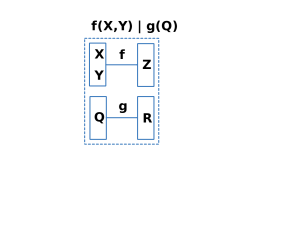
\includegraphics[width=0.1\textwidth]{figs/parallel.png}
  \caption{Parallel Model Composition in AMIDOL}
  \label{Fig:Parallel}
\end{figure}

Parallel composition is accomplished by sharing no state variables,
resulting in the diagram shown in \ref{Fig:Parallel}.  This has the
effect of taking the union of input and output objects of both
morphisms, and treating the new parallel composition as a morphism
between these unions.  While seemingly simple, this construct allows
for a richer set of serial compositions by altering the apparent input
and output model signatures of the new composed models to potential
match other models with which it can then be composed.

\begin{figure}
  \centering
  \includegraphics[width=0.2\textwidth]{figs/serial.png}
  \caption{Serial Model Composition in AMIDOL}
  \label{Fig:Serial}
\end{figure}

Serial composition, shown in Figure \ref{Fig:Serial}, is accomplished by taking the disjoint
union of two open models in AMIDOL's IR, $P: X \rightarrow Y$, and
$Q: Y \rightarrow Z$ resulting in $P+Q: X \rightarrow Z$, sharing all
similar states in the objects $Y$ belonging to $P$ and $Q$.

\begin{figure}
  \centering
  \includegraphics[width=0.2\textwidth]{figs/substitution.png}
  \caption{AMIDOL Architecture}
  \label{Fig:Sub}
\end{figure}

Lastly, AMIDOL implements substititional composition using the
double-push out rule shown in Figure \ref{Fig:Sub}, implementing the
double-push out graph rewriting mechanism.  Substitution of subgraphs
(of events and states) with other compatible subgraphs
provides a mechanism for quickly swapping out sub-models used in a
bigger model (for instance: changing an SIR model into an SEIR one).
The substitional transformation requires a user to give an example of
the initial model, the model invariants, and the resulting new model
to be obtained via substition.  While semantically valid, it presents
some possible issues as it is entirely possible for subgraph
substitution to accidentally “break” some other part of the
model. Consider the case of swapping an SIR sub-model for an SEIR
sub-model: elsewhere in the larger model, uses of $S + I + R$ probably
indicated “total population” and should be replaced with $S + I + E +
R$.  To address this issue we are focusing our future work on
providing a mechanism for building up symbolic expressions
alleviating the pain of “refactoring” after
substitution.

\end{document}